\documentclass[a4paper,12pt]{article}
\usepackage{fancyhdr}
\usepackage{geometry}
\geometry{hmargin=2.5cm,vmargin=1.5cm}
\usepackage[utf8]{inputenc}%encodage des caractères    
                         
\usepackage[T1]{fontenc}%encodage de la police    
                              
\usepackage[french]{babel}%langue française
\usepackage{float}



\frenchbsetup{StandardLists=true} % à inclure si on utilise \usepackage[french]{babel}

\usepackage{enumitem}

\usepackage[linesnumbered,ruled,french,onelanguage]{algorithm2e}
\usepackage{listings}
\lstset{language=Java,
  showspaces=false,
  showtabs=false,
  breaklines=true,
  showstringspaces=false,
  breakatwhitespace=true,
  commentstyle=\color{pgreen},
  keywordstyle=\color{pblue},
  stringstyle=\color{pred},
  basicstyle=\ttfamily,
  moredelim=[il][\textcolor{pgrey}]{$$},
  moredelim=[is][\textcolor{pgrey}]{\%\%}{\%\%}
}
	
\usepackage{color}

\usepackage{hyperref}
\usepackage{amsmath}

% Pour l'inclusion des diagrammes UML                                           
\usepackage{graphicx}
\newcommand{\umlscale}{0.4}

% Écriture des noms de classes, etc.                                            
\newcommand{\packagename}[1]{\texttt{#1}}
\newcommand{\classname}[1]{\texttt{#1}}
\newcommand{\methodname}[1]{\texttt{#1}}
\newcommand{\HRule}{\rule{\linewidth}{0.5mm}}
\makeatletter
\renewcommand\paragraph{\@startsection{paragraph}{4}{\z@}%
% display heading, like subsubsection
                                     {-3.25ex\@plus -1ex \@minus -.2ex}%
                                     {1.5ex \@plus .2ex}%
                                     {\normalfont\normalsize\bfseries}}
 \setcounter{secnumdepth}{4}
\makeatother

\SetAlFnt{\small\sffamily}


% Inclure des sections ou sous-sections dans le sommaire
\newcommand{\nocontentsline}[3]{}
\newcommand{\tocless}[2]{\bgroup\let\addcontentsline=\nocontentsline#1{#2}\egroup}
%%%% un bug dans la version française de algorithm2e : pas de traduction de output sans les lignes ci-dessous
\makeatletter 
\g@addto@macro{\@algocf@init}{\SetKwInput{KwOut}{Sortie}} 
\makeatother
%%%%%



\begin{document}
\thispagestyle{empty}
%Page de garde
\begin{titlepage}
	%haut de la page
	\begin{center}
		
\includegraphics[scale=0.2]{Images/logos-Marianne-UNICAEN-scaled.jpg}\\[1.5cm]

		%type de document : rapport
		\textsc{\Large Rapport de Projet}\\[1.5cm]

		%Nom du projet
		\HRule \\[0.4cm]
		{
		\Large \bfseries Étude des performances des algorithmes Max$^n$ et paranoid 
		pour la prise de décision dans le jeu de Tron Multijoueur
		 \\[0.2cm]
		}
		\HRule \\[0.5cm]
	\end{center}

	%Equipe Developpement
	\begin{minipage}[c]{0.5\linewidth}
		%Membres du groupes
		\begin{flushleft}
			\underline{Equipe de développement}: \\[0.5cm]
			A. Catherine ATTY\\[0.2cm]
			Sékou DOUMBOUYA\\[0.2cm]
			Manne Emile KITSOUKOU\\[0.2cm]
			Amirath Fara OROU-GUIDOU\\[0.5cm]
			%OROU-GUIDOU Amirath Fara\\[0.5cm]
			%Info sur la formation
			\underline{Parcours} : Licence 3 Informatique\\[0.2cm]
			\underline{Groupe} : 2B\\
		\end{flushleft}
	\end{minipage}

	%Superviseurs
	\begin{minipage}[c]{\linewidth}
		\begin{flushright}
			\underline{Sous la supervison} :\\[0.5cm]
			LEHEMBRE Etienne\\[0.2cm]
		\end{flushright}
	\end{minipage}\\[0.7cm]

	%bas de la page de garde
	%\center Avril 2022
	\center \today
\end{titlepage}
\thispagestyle{empty}
%page de sommaire
\tableofcontents
\newpage

%L'ecriture du document commence ici

\setcounter{page}{1}
\addcontentsline{toc}{section}{Introduction}
\section*{Introduction}
\label{sec:intro}
La \textbf{théorie des jeux} et l'\textbf{intelligence artificielle} sont deux(2) domaines 
interconnectés qui ont connu une évolution fulgurante ces dernières années. La théorie des 
jeux est une branche des mathématiques qui se concentre sur l'analyse de la prise de décision 
stratégique dans des situations où de multiples acteurs interagissent et ont des intérêts 
contradictoires. Elle fournit un cadre pour l'analyse des choix des agents rationnels\footnote{Un 
agent rationnel est une entité qui vise toujours à réaliser des actions optimales sur la base de 
prémisses et d’informations données.} et la prédiction de leurs résultats dans différents scénarios. 
En revanche, l'intelligence artificielle vise à doter les machines de la capacité d'imiter le 
comportement humain. Elle repose sur diverses techniques, telles que les algorithmes de recherche, 
l'apprentissage automatique et le traitement du langage naturel, pour simuler un comportement 
intelligent et prendre des décisions sur la base de données et de règles.\\

Le mariage entre la théorie des jeux et l'intelligence artificielle a conduit à de nombreuses 
applications, telles que les moteurs d'échecs, les robots de poker et les systèmes de recommandation. 
De plus, cette alliance a permis l'émergence de nouvelles voies de recherche, notamment les systèmes 
multi-agents, l'apprentissage par renforcement et la théorie du choix social.\\ 

Dans ce projet, nous avons l'ambition d'utiliser la théorie des jeux et l'intelligence artificielle 
pour mettre en œuvre et étudier le \textbf{jeu de Tron} avec plusieurs joueurs et différentes stratégies. Le jeu de Tron 
est un jeu multijoueur captivant inspiré du célèbre jeu \textbf{Snake}\footnote{Le snake, de 
l’anglais signifiant « serpent », est un genre de jeu vidéo où le joueur contrôle un serpent 
qui s’agrandit au fur et à mesure de la progression du jeu, créant ainsi des obstacles pour le joueur}.
Dans ce dernier, les joueurs contrôlent un point qui se déplace sur une grille de taille fixe et laisse 
derrière lui un mur infranchissable à chaque déplacement. Le but est d'être le dernier joueur debout 
en évitant les collisions avec les murs, les bords et les trajectoires des adversaires. Ce jeu 
présente plusieurs défis pour l'analyse, tels que l'observabilité partielle, les mouvements 
simultanés et l'incertitude quant aux intentions des adversaires. Pour relever ces défis, les 
chercheurs ont proposé différents algorithmes, tels que $negamax$ avec élagage $alpha-beta$, 
recherche arborescente de $Monte$ $Carlo$ et $Max^n$. Toutefois, l'ajout de plusieurs joueurs et équipes 
crée de nouvelles dimensions de complexité et de stratégie.\\

L'objectif de ce projet est d'étudier l'efficacité de différents algorithmes de jeu en évaluant les 
performances d'abord d'un agent solitaire, puis d'un agent multi-joueur. Pour ce faire, 
une analyse statistique sera effectuée dans diverses configurations de jeu. Ainsi, 
nous pourrons déterminer les algorithmes les plus efficaces et les plus performants.\\

Dans ce document, nous introduirons d'abord le jeu de Tron. Puis, nous exposerons la structure du projet et 
les phases successives de son élaboration. Ultérieurement, nous approfondirons les algorithmes de jeu employés 
et l'architecture globale du projet. Finalement, nous présenterons les constatations dérivées de notre évaluation 
statistique et tirerons des conclusions sur la performance des algorithmes.

\newpage
\section[Jeu de Tron]{Jeu de Tron : Un jeu multijoueur captivant}
\label{sec:jeu_tron}
\tocless\subsection{Desciption du jeu}
Film iconique des années 1980, \textbf{Tron} est une science-fiction américain réalisé par
Steven Lisberger au sein de l'entreprise Walt Disney Pictures. Ce dernier met en scène un jeu dans 
un monde virtuel où des motos futuristes se déplacent à une vitesse constante, n'effectuant que des 
virages à angle droit\footnote{Les virages à angle droit sont des virages où la nouvelle direction 
est perpendiculaire à la direction précédente.} 
\begin{figure}[h!]
	\centering
	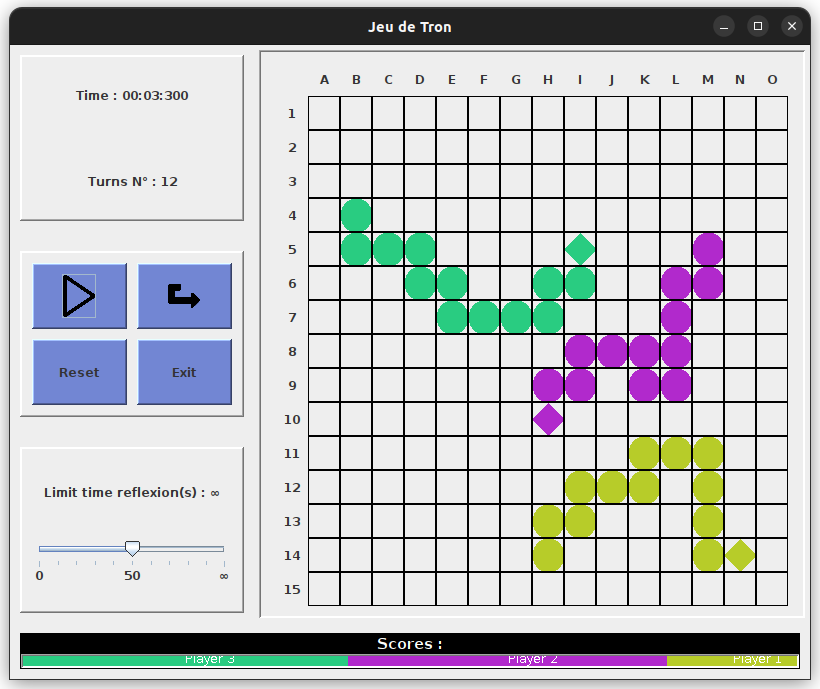
\includegraphics[scale=0.35]{Images/jeu-tron.png}
	\caption{Jeu de Tron}
	\label{fig:jeu-tron}
\end{figure}
et laissant derrière elles des trainées solides. Ainsi,
au fur et à mesure que le jeu avance, le plateau se remplit de murs et finalement un ou plusieurs
joueurs se retrouvent coincés dans un cul-de-sac. Le but du jeu est de survivre le plus longtemps et 
d'être le dernier survivant. Ce jeu est devenu très populaire et a ensuite été implémenté sur diverses
plateformes et diverses versions.\\
\tocless\subsection{Analyse mathématiques du jeu}
\textbf{Tron} est un jeu se jouant sur une grille de taille $N\times M$ avec $N$ et $M$ entiers positifs. Chaque 
cellule de la grille peut être \texttt{vide} ou \texttt{occupée} par un joueur. Généralement, la grille 
considérée est carrée, c'est à dire $N=M$. C'est un jeu multijoueur dans lequel les $K$ joueurs, à 
chaque tour, font un choix:
\begin{itemize}
	\item \texttt{continuer} dans la même direction
	\item \texttt{tourner} à $90^{\circ}$ à gauche ou à droite
\end{itemize}
Un joueur ne peut pas s'arreter et doit toujours se déplacer. C'est un jeu assez rapide, car les
joueurs se déplacent à une vitesse constante($\approx 100ms$ par tour). Tous les choix sont fait 
de manière simultanée ce qui rend le jeu très dynamique et complexifie l'anticipation des mouvements
des adversaires. Le jeu se finit avec 2 états possibles:
\begin{itemize}
	\item \texttt{victoire} d'un joueur, si il est le dernier survivant
	\item \texttt{nulle} si tous les joueurs sont éliminés
\end{itemize}

Plus en détail, à chaque sequence discrète de temps $t=0,1,2,...$, les joueurs $i=1,2,...,K$ reçoivent 
une même représentaion $s_t \in S$ de l'état du jeu, où $S$ est l'espace des états possibles. 
%Integrer un fichier
\begin{figure}
	\centering
	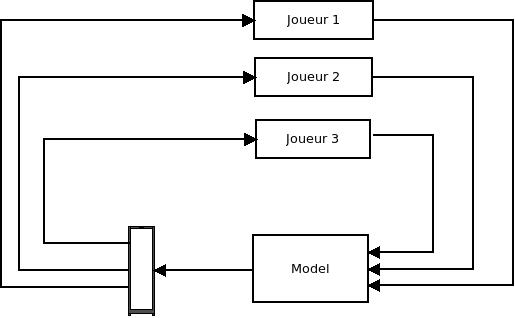
\includegraphics[scale=0.4]{Images/interraction_model.jpeg}
	\caption{Modèle d'interraction entre 3 joueurs}
	\label{fig:modele-interraction}
\end{figure}
En fonction de l'état $s_t$, chaque joueur $i$ choisit une action $a_{i,t} \in A_i(s_t)$, où $A_i(s_t)$
est l'espace des actions possibles pour le joueur $i$ dans l'état $s_t$. Ainsi, chaque joueur $i$. Comme conséquence,
chaque joueur $i$ reçoit une nouvelle représentation $s_{t+1} \in S$ de l'état courant du jeu.\ref{fig:modele-interraction}


Ainsi le jeu de Tron est un jeu ayant une longueur fini. En effet, le nombre d'étape nécessaire 
pour terminer le jeu est majoré par :
\begin{equation}
	\label{eq:nb-etapes}
	\frac{N\times M}{K}
\end{equation}
où $N$(resp. $M$) est la taille de la grille en largeur (resp. en hauteur) et $K$ est le nombre de joueurs.\\
Toutefois en pratique, le jeu peut se terminer plus ou moins rapidement en fonction de la stratégie
des joueurs.

\section{Problématique et hypothèses de recherche}
\label{sec:problematique}
\tocless\subsection{Problemématique de recherche}
Le jeu de Tron est un jeu multijoueur complexes qui implique la prise de décision stratégique,
la coordination et la compétition. L'un des principaux défis de ce jeu est d'anticiper les mouvements
des adversaires et de concevoir des stratégies efficaces qui peuvent maximiser les chances de survie et
de victoire d'un joueur. Cependant la stratégie optimale n'est pas toujours évidente, car elle dépend
de divers facteurs. En effet, la taille de la grille, le nombre d'adversaires, la profondeur de recherche, 
la stratégie des adversaires et les ressources de calcul sont autant de facteurs qui peuvent influencer
les performances d'un joueur. Ainsi, le projet vise à étudier l'efficacité de différents algorithmes de jeu
à travers l'analyse de l'impact de ces divers facteurs sur les performances des joueurs.\\

\tocless\subsection{Hypothèses de recherche}
Pour répondre à cette problématique, diverses hypothèses de recherche ont été formulées:
\begin{itemize}
	\item La performance des stratégies s'améliore avec la profondeur de recherche accordée à l'agent.
	\item L'efficacité des algorithmes se réduisent avec l'augmentation du nombre d'adversaires.
	\item Il existe une taille maximale de grille pour laquelle après dépassement, les performances des stratégies diminuent.
\end{itemize}
Ces hypothèses guideront les expérimentations, l'analyse des données et l'interpretation des résultats, et 
seront utilisées pour évaluer la pertinence des algorithmes de jeu.

\section{Etat de l'art : théorie des jeux et Recherche adversarial}
\label{sec:etat_art}
Le jeu Tron appartient à un genre prisé de jeux d'arcade basés sur la navigation d'un protagoniste à travers une grille labyrinthique. 
Depuis leur apparition, ces jeux ont évolué, intégrant désormais des fonctionnalités multijoueurs et des mécaniques de jeu plus élaborées. 
L'application de l'intelligence artificielle (IA) et de la théorie des jeux dans l'analyse de ces jeux a suscité un intérêt croissant, 
poussant les chercheurs à développer divers algorithmes et stratégies pour optimiser les performances des joueurs. Dans ce qui suit,
nous présentons les algorithmes et stratégies prédominants dans le jeu de Tron, passons en revue la littérature existante concernant l'application de l'IA 
et de la théorie des jeux, mettons en évidence les avantages et les limites des différentes approches et identifiant les lacunes dans l'état actuel 
de la recherche.

\tocless\subsection{Théorie des jeux}
La théorie des jeux a été appliquée au jeu de Tron pour analyser la prise de décision stratégique de plusieurs joueurs 
et développer des stratégies de jeu optimales. Les recherches précédentes se sont concentrées sur l'utilisation de différents 
concepts de la théorie des jeux, tel que les équilibres de Nash et les stratégies mixtes, pour modéliser le comportement des 
joueurs et prédire leurs mouvements. Certaines études ont également exploré l'utilisation 
d'heuristique pour guider les joueurs vers des stratégies optimales dans divers scénarios.\\


En gandre partie, les études se sont concentrées sur l'examen de l'algorithme de recherche arborescente de $Monte$ $Carlo$ (MCTS). 
Des travaux tels que ceux de \textbf{Perick} \textbf{et al.} \cite{perick2012comparison} ont comparé différentes méthodes de sélection 
pour optimiser les performances de l'algorithme. Il en découle que l'adoption d'une stratégie de sélection spécifique peut améliorer les résultats de l'algorithme. 
De plus, d'autres recherches, comme celle de \textbf{Den} \textbf{et al.} \cite{den2011monte} ont exploré diverses heuristiques pour accroître l'efficacité de
ces algorithmes. Ainsi, l'emploi d'une heuristique fondée sur l'estimation de l'espace libre constitue un bon indicateur de la qualité d'une action.\\

De plus, des travaux connexes ont été menées  en utilisant des algorithmes de recherche adversarial($minimax$, $alpha$-$beta$, $negamax$...). 
C'est le cas des travaux de \textbf{Boin}\cite{boincs221} dans lequel il présente divers versions de l'algorithme $minimax$ et des 
heuristiques pour améliorer les performances de l'algorithme. Un autre article facinant est celui réalisé par le vainqueur de 
\textbf{Google IA Challenge} \cite{sloane_2010} qui a utilisé un algorithme de recherche adversarial pour sortir victorieux de ce Challenge.
Il y montre et explique les différentes étapes de son travail, notamment celui sur l'implémentation des heuristiques qui apporte une 
amélioration significative des performances de l'algorithme.\\


\tocless\subsection{Recherche adversarial multijoueur}
La recherche adversarial est une technique fréquemment employée pour modéliser le comportement des participants dans les 
environnements multi-agents. Cela englobe l'analyse des algorithmes et des stratégies pour des scénarios 
impliquant plus de deux acteurs. Deux approches principales existent pour aborder ce défi, notamment l'application des algorithmes suivants : 
\begin{itemize}
	\item \textbf{Max}$^n$
	\item \textbf{Paranoid}
\end{itemize}
Ces algorithmes ont fait leur preuve dans le domaine des jeux multijoueurs
et ont été largement utilisés pour analyser les stratégies de jeu optimales. En effet la recherche réalisé par \cite{nathan} ont montré que l'algorithme paranoïaque 
est une option viable pour les jeux multijoueurs, puisqu'il surpasse systématiquement l'algorithme maxn au jeu de dames et obtient des résultats légèrement meilleurs au jeu de cœur. Cependant, l'algorithme maxn reste compétitif dans les jeux où il peut élaguer. Dans l'ensemble, nous concluons que l'algorithme paranoïaque est supérieur dans les jeux où l'algorithme maxn est contraint d'effectuer une recherche par force brute



\section{Organisation et planification}
\label{sec:organisation}
Afin d'accomplir ce projet avec succès, nous avons opté pour une approche intégrant des
\textbf{analyses théoriques}, la \textbf{mise en oeuvre d'algorithmes} et des \textbf{évaluations
empiriques}\footnote{L'évaluation empirique désigne le processus consistant à utiliser des 
expériences, des mesures et des observations pour évaluer la performance ou l'efficacité 
d'un système ou d'une approche particulière}. Pour ce faire, nous devrions dans un premier temps
fixer des objectifs clairs et définir les différentes étapes de notre travail. Ensuite, nous devrions
nous pencher sur la relation de ces derniers en s'organisant et en planifiant notre travail.

\subsection{Etapes du projet}
Notre travail est divisé en trois grandes étapes principales :
\begin{itemize}
	\item \textbf{Planification} :  Définition des questions de recherche, formulation des hypothèses, Recherche bibliographique, choix de l'approche méthodologique et modèlisation du jeu.
	\item \textbf{Implémentation et Développement}: Développement du jeu, implémentation des algorithmes de recherche adversarial et des heuristiques, préparation des données et des expériences.
	\item \textbf{Evaluation et Analyse}: Analyse des résultats, interprétation des résultats et discussion des résultats.
\end{itemize}
Chacune des étapes comporte des objectifs et tâches spécifiques dont leur accomplissement est 
nécessaire pour le succès du projet.

\subsection{Gestion du projet}

Pour le bon déroulement du projet, nous avons décidé d'organiser globalement divers parties implémenter par chaque membre du groupe. 
Ainsi, nous avons décidé de nous répartir les tâches suivantes:
\begin{itemize}
	\item \textbf{Manne}: Implémentation du modèle de jeu et des heuristiques
	\item \textbf{Amirath}: Implémentation des algorithmes de recherche adversarial ($Max^n$ et $Paranoid$)
	\item \textbf{Catherine}: Implémentation des algorithmes de recherche adversarial et mise en place de la plateforme de test
	\item \textbf{Sekou} : Réalisation de l'interface graphique
\end{itemize}
En outre, nous avons décidé que chacun des membres du groupe devrait participer à l'analyse des résultats.
\subsection{Planification du travail}
Le diagramme de Gantt\footnote{Diagramme de Gantt est un diagramme de type barre qui permet de représenter graphiquement l'avancement d'un projet.} ci-dessous représente la planification du travail.
\begin{figure}[!ht]
	\centering
	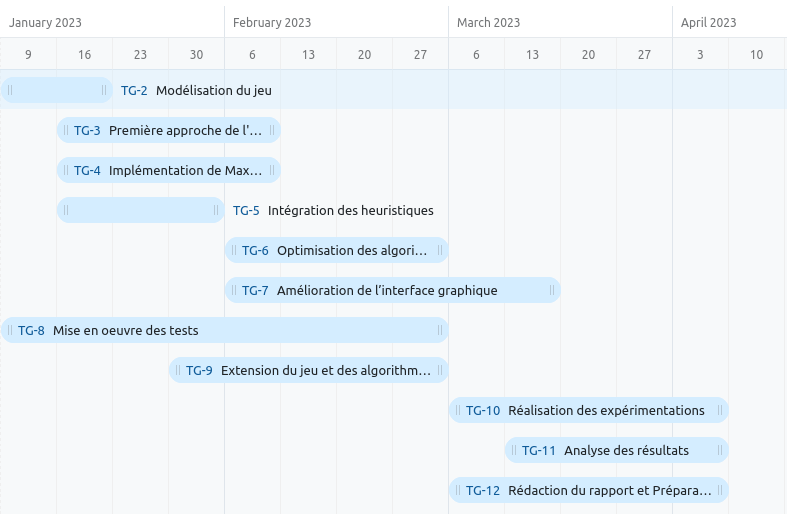
\includegraphics[scale=0.5]{Images/gant.png}
	\caption{Diagramme de Gantt}
	\label{fig:gantt}
\end{figure}
Nous avons décidé de travailler sur le projet en trois phases, à savoir:
\begin{itemize}
	\item \textbf{Phase 1}: Développement de l'environnement de jeu, implémentation des heuristiques, des algorithmes de recherche adversarial et mise en place de la plateforme de test
	\item \textbf{Phase 2}: Amélioration de l'environnement de jeu, algorithmes et extensions des algorithmes à la version multi-joueurs
	\item \textbf{Phase 3}: Réalisation des expériences et analyse des résultats
\end{itemize}


\section[Analyse et Démonstration des algorithmes]{Analyse et Démonstration des algorithmes : Les heuristiques}
\label{sec:analyse}
Dans le cadre de ce projet, différentes techniques heuristiques ont été utilisées pour améliorer l'algorithme de prise de décision. 
Nous avons pris la décision de nous concentrer exclusivement sur les heuristiques basées sur l'occupation de l'espace. Ces heuristiques sont particulièrement 
adaptées pour faciliter l'analyse des positions de jeu et l'évaluation de leur qualité. 

\subsection{OpenSpace}
L'heuristique \textbf{OpenSpace} est une technique simple basée sur la comptabilisation du nombre de cases vides entourant 
un joueur donné. Elle se fonde uniquement sur la position de ce joueur et ne prend pas en considération la position des 
autres joueurs.

\tocless\subsubsection{Implémentation}
Son implémentation consiste à calculer le nombre de cases vides situées autour d'un joueur donné, à partir d'un état de jeu spécifique.\\

\begin{algorithm}[H]
	\caption{OpenSpace}
	\label{alg:openspace}
	\DontPrintSemicolon
	\KwIn{$state$ : état du jeu}
	\KwOut{$scores$ : score de l'état}
	$scores \gets \{\}$\;
	\For{$player \in state.players$}{
		$score \gets 0$\;
		\For{$neighbor \in state.neighbors(player)$}{
			\If{$neighbor \in state.empty$}{
				$score \gets score + 1$\;
			}
		}
		$scores[player] \gets score$\;
	}
	\Return $scores$\;
\end{algorithm}

\tocless\subsubsection{Complexité}
L'algorithme \textbf{OpenSpace}~\ref{alg:openspace} a une complexité temporelle qui dépend uniquement du nombre de joueurs dans le jeu.\\

En effet la boucle extérieure de l'algorithme parcourt tous les joueurs présents dans l'état de jeu, ce qui prend un temps 
proportionnel à N, où N est le nombre de joueurs. De plus la boucle intérieure itère sur les quatres(4) voisins de chaque joueur, et 
la vérification de la liberté de chaque voisin(voir la ligne 5~\ref{alg:openspace}) se fait en temps constant($\mathcal{O}(1)$).\\

Par conséquent, la complexité de l'algorithme \textbf{Openspace} est de l'ordre de $\mathcal{O}(N)$, 
ce qui peut être considéré comme linéaire en fonction du nombre de joueurs.\\

\subsection{GASLAP}
\textbf{GASLAP} abréviation de "\textbf{G}o \textbf{AS} \textbf{L}ong \textbf{A}s \textbf{P}ossible" est une approche 
qui consiste à calculer la distance maximale qu'un joueur peut parcourir à partir de sa position de départ dans une 
direction donnée, sans rencontrer d'obstacles. Cette méthode permet de prioriser les mouvements qui permettent au 
joueur de se déplacer le plus loin possible dans la direction choisie, tout en évitant les déplacements inutiles 
et en maximisant l'efficacité des mouvements.

\tocless\subsubsection{Implémentation}
Cette approche s'appuie sur la détermination du nombre de cases vides situées dans la direction choisie par le joueur.\\

\begin{algorithm}[H]
	\caption{GASLAP}
	\label{alg:gaslap}
	\DontPrintSemicolon
	\KwIn{$state$ : état du jeu}
	\KwOut{$scores$ : score de l'état}
	$scores \gets \{\}$\;
	\For{$player \in state.players$}{
		$score \gets 0$\;
		$direction \gets state.direction(player)$\;
		$position \gets player.position$\;
		\While{$position \in state.empty$}{
			$position \gets position + direction$\;
			$score \gets score + 1$\;
		}
		$scores[player] \gets score$\;
	}
	\Return $scores$\;
\end{algorithm}

\tocless\subsubsection{Complexité}
Étant donné que le jeu se déroule sur une grille carrée de taille fixe $n \times n$,un joueur ne peut se déplacer dans une même direction que
$n-1$ fois. Ainsi, la complexité de la boucle intérieure(boucle \textbf{While}) est de l'ordre de $\mathcal{O}(n)$. De plus la boucle extérieure
(boucle \textbf{For}) parcourt tous les joueurs présents dans l'état de jeu, ce qui prend un temps proportionnel à $J$, où $J$ est le nombre de joueurs.\\

Par conséquent, la complexité de l'algorithme \textbf{GASLAP} est de l'ordre de $\mathcal{O}(J \times n)$, ce qui peut être considéré comme
linéaire en fonction du nombre de joueurs car $n$ est une constante.\\

\subsection{Voronoï}
Le diagramme de \textbf{Voronoï} est une technique mathématique qui permet de diviser l'espace en régions distinctes en 
fonction de la proximité de points spécifiques. Dans le cadre de ce projet, nous avons utilisé cette technique pour 
déterminer les zones d'influence\footnote{Zone d'influence est la zone pour laquelle un joueur peut atteindre en premier à partir de sa position de départ.} 
des joueurs.
\tocless\subsubsection{Implémentation}
Pour mettre en œuvre cette technique, nous commençons par calculer la distance entre le joueur et toutes les autres 
cases vides\footnote{Case vide est une case qui n'est pas occupée par un joueur.} de la grille. Pour ce faire, nous adaptons 
les principes de l'algorithme de \textbf{Dijkstra} à notre cas spécifique(voir algorithme \ref{algo:distance}).\\

\begin{algorithm}[H]
	\caption{Détermination de la distance entre le joueur et les cases vides}
	\label{algo:distance}
	\DontPrintSemicolon
	\SetKwComment{Comment}{/* }{ */}
	\KwIn{$initial\_position$ : Position initial du joueur, $positions\_vides$ : Ensemble des positions des cases vides}
	\KwOut{$distances$ : Dictionnaire contenant les distances entre le joueur et les cases vides}
	$distances \gets \{\}$\;
	$queue \gets \{\}$\;
	\ForEach{$position\_vide \in positions\_vides$}{
		$distances[position\_vide] \gets \infty$\;
	}
	$distances[initial\_position] \gets 0$\;
	$queue \gets queue \cup \{initial\_position\}$\;
	\While{$queue \neq \{\}$}{
		$position \gets queue[0]$ \;
		$queue \gets queue \setminus \{position\}$\;
		\ForEach{$adjacent \in get\_adjacents(position)$}{
			\If{$distances[adjacent] > distances[position] + 1$}{
				$distances[adjacent] \gets distances[position] + 1$\;
				$queue \gets queue \cup \{adjacent\}$\;
			}
		}
	}
	\Return $distances$\;
\end{algorithm}

Après avoir calculé les distances entre chaque joueur et les cases vides à l'aide de l'algorithm \ref{algo:distance}, 
nous utilisons ces informations pour déterminer les zones d'influence de chaque joueur en ajoutant les cases vides les plus 
proches de lui, et nous obtenons la taille de ces zones d'influence en utilisant la méthode décrite dans l'algorithme \ref{algo:voronoï}.\\

\begin{algorithm}[H]
	\caption{Détermination de la zone d'influence d'un joueur}
	\label{algo:voronoï}
	\DontPrintSemicolon
	\SetKwComment{Comment}{/* }{ */}
	\KwIn{$state$ : Etat courant du jeu}
	\KwOut{$zones\_influence$ : Dictionnaire contenant la taille de la zone d'influence de chaque joueur}
	$zones\_influence \gets \{\}$\;
	$distances \gets \{\}$\;
	\ForEach{$player \in state.players$}{
		$zones\_influence[player] \gets 0$\;
		$distances[player] \gets distance(player.position, state.vide\_positions)$\;
	}
	\ForEach{$position\_vide \in state.vide\_positions$}{
		$min\_distance \gets \infty$\;
		$min\_player \gets None$\;
		\ForEach{$player \in state.players$}{
			\If{$distances[player][position\_vide] < min\_distance$}{
				$min\_distance \gets distances[player][position\_vide]$ \;
				$min\_player \gets player$\;
			}
			\ElseIf{$distances[player][position\_vide] == min\_distance$}{
				$min\_player \gets None$\;
			}
		}
		\If{$min\_player \neq None$}{
			$zones\_influence[min\_player] \gets zones\_influence[min\_player] + 1$\;
		}
	}
	\Return $zones\_influence$\;
\end{algorithm}

\tocless\subsubsection{Complexité}
Étant donné que l'algorithm \textbf{Voronoï}~\ref{algo:voronoï} est basé sur l'utilisation de l'algorithme de \textbf{distance}~\ref{algo:distance}, 
il existe un lien direct entre la complexité de ces deux algorithmes. \\

En effet, l'algorithme de \textbf{distance}~\ref{algo:distance} est basé sur l'algorithme de \textbf{Dijkstra} qui est un algorithme ayant une complexité
de l'ordre de $\mathcal{O}{(|A| + |S|log|S|)}$ où $A$ est l'ensemble des arêtes \footnote{Arête est une liaison entre deux cases.} de la grille et 
$S$ est l'ensemble des cases vide de la grille. Vu que l'on itère $J$ fois sur l'algorithme de \textbf{distance}~\ref{algo:distance} où $J$ est le nombre de joueurs,
la complexité de la première partie de l'algorithme \textbf{Voronoï}~\ref{algo:voronoï}~(ligne 3-6) est de l'ordre de $\mathcal{O}{(J(|A| + |S|log|S|))}$. La deuxième partie de l'algorithme
\textbf{Voronoï}~\ref{algo:voronoï}~(ligne 7-15) est basée sur une double itération entre les cases vides et les joueurs, la complexité de cette partie est donc de l'ordre de
$\mathcal{O}{(|S|J)}$. \\

La complexité totale de l'algorithme \textbf{Voronoï}~\ref{algo:voronoï} est donc de l'ordre de $\mathcal{O}{(J(|A| + |S|log|S|) + |S|J)}$.\\

Toutefois, en fonction de l'état de la grille, on distingue deux cas où l'on peut majoré beaucoup plus efficacement la complexité de l'algorithme \textbf{Voronoï}~\ref{algo:voronoï}:
\begin{itemize}
	\item $|S| \gg |A|$ : Dans ce cas, on peut majorer la complexité de l'algorithme \textbf{Voronoï}~\ref{algo:voronoï} en $\mathcal{O}{(J|S|log|S|)}$.
	\item $|S| \ll |A|$ : Dans ce cas, on peut majorer la complexité de l'algorithme \textbf{Voronoï}~\ref{algo:voronoï} en $\mathcal{O}{(J|A|)}$.
\end{itemize}
C'est deux(2) cas sont ceux qui sont le plus souvent rencontrés dans le jeu de \textbf{Tron}.\\

\subsection{Checker}
Compte tenu de la structure du jeu qui se joue sur une grille, nous pouvons considérer cette grille comme un échiquier, où les cases sont alternativement 
blanches et noires. En conséquence, un joueur ne peut se déplacer que d'une case blanche à une case noire ou vice versa. Ainsi, en utilisant l'algorithme 
\textbf{Voronoï}~\ref{algo:voronoï}, nous pouvons éliminer les cases blanches et noires excédentaires qui se trouvent dans la zone d'influence d'un joueur. 
Cela nous permet d'obtenir une limite supérieure plus précise de la zone d'influence d'un joueur.

\tocless\subsubsection{Implémentation}
L'algorithme \textbf{Checker}~\ref{algo:checker} est découle du développement réalisé sur celui de voronoï, une différence notable est que dans le case 
du \textbf{Checker}, nous comptons le nombre de cases blanches et noires dans la zone d'influence d'un joueur, ce qui permet d'en réduire le surplus.\\

\begin{algorithm}[H]
	\caption{Détermination de la zone d'influence d'un joueur}
	\label{algo:checker}
	\DontPrintSemicolon
	\SetKwComment{Comment}{/* }{ */}
	\KwIn{$state$ : Etat courant du jeu}
	\KwOut{$zones\_influence$ : Dictionnaire contenant la taille de la zone d'influence de chaque joueur}
	$zones\_influence \gets \{\}$\;
	$distances \gets \{\}$\;
	$count_{white} \gets 0$\;
	$count_{black} \gets 0$\;
	\For{$player \in state.players$}{
		$distances[player] \gets distance(state, player)$\;
		$zones\_influence[player] \gets 0$\;
		$count_{white}[player] \gets 0$\;
		$count_{black}[player] \gets 0$\;
	}
	\ForEach{$position\_vide \in state.vide\_positions$}{
		$min\_player \gets None$\;
		$min\_distance \gets \infty$\;
		\For{$player \in state.players$}{
			\If{$distances[player][position\_vide] < min\_distance$}{
				$min\_player \gets player$\;
				$min\_distance \gets distances[player][position\_vide]$ \Comment{On récupère le joueur le plus proche de la case vide}
			}
			\ElseIf{$distances[player][position\_vide] == min\_distance$}{
				$min\_player \gets None$\;
				$min\_distance \gets \infty$\;
			}
		}

		\If{$min\_player != None$}{
			$zones\_influence[min\_player] \gets zones\_influence[min\_player] + 1$\;
			\If{$position\_vide.color == 'white'$}{
				$count_{white}[min\_player] \gets count_{white}[min\_player] + 1$\;
			}
			\Else{
				$count_{black}[min\_player] \gets count_{black}[min\_player] + 1$\;
			}
			$zones\_influence[min\_player] \gets zones\_influence[min\_player] + 1$\;
		}
	}
	\For{$player \in state.players$}{
		$surplus \gets |count_{white}[player] - count_{black}[player]|$\;
		$zones\_influence[player] \gets zones\_influence[player] - surplus$\;
	}
	\Return $zones\_influence$\;
\end{algorithm}

\tocless\subsubsection{Complexité}
La complexité dans le pire des cas de l'algorithme \textbf{Checker}~\ref{algo:checker} est du même ordre que celle de l'algorithme \textbf{Voronoï}~\ref{algo:voronoï},
c'est à dire $\mathcal{O}{(J(|A| + |S|log|S|))}$. En effet, l'algorithme \textbf{Checker}~\ref{algo:checker} est une extension de l'algorithme \textbf{Voronoï}~\ref{algo:voronoï}. Cette 
extension permet de trouver une limite supérieure plus précise de la zone d'influence d'un joueur.\\




\section{Architecture du projet}
\label{sec:architecture}
Notre projet est basé sur l'architecture logicielle MVC (Modèle-Vue-Contrôleur) qui permet de séparer la logique métier de la présentation.
Nous avons ainsi identifié 4 modules principaux(voir figure \ref{fig:architecture}):
\begin{figure}[H]
	\centering
	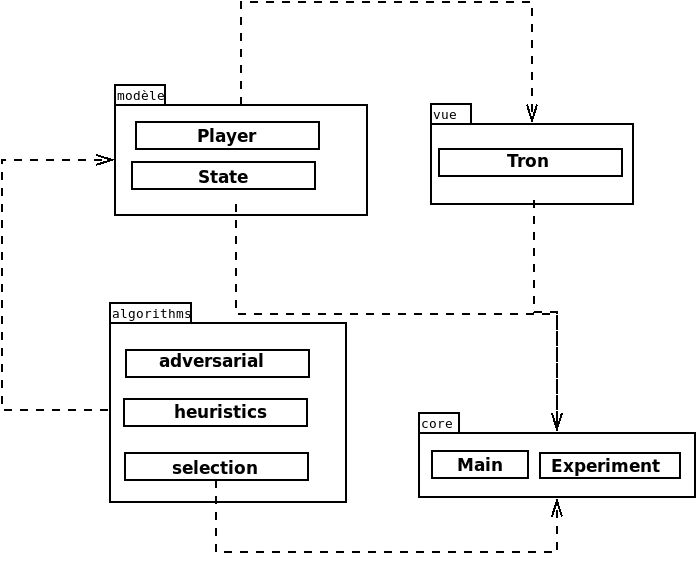
\includegraphics[scale=0.4]{diagrames/architecture}
	\caption{Architecture du projet}
	\label{fig:architecture}
\end{figure}

\begin{itemize}
	\item \textbf{Modèle} : Il contient les classes qui représentent les différents éléments du jeu comme les joueurs, la grille de jeu, etc. Il gère également les règles du jeu et les interactions entre les différents éléments.
	\item \textbf{Vue} : Il est responsable de l'affichage graphique du jeu et des interactions utilisateur. Il est constitué d'une interface utilisateur (UI) qui permet à l'utilisateur de jouer et de visualiser les différentes informations du jeu.
	\item \textbf{Core} : Contient l'ensemble des classes executables qui permettent de lancer le jeu.
	\item \textbf{algorithms}: Il contient l'ensemble des algorithmes de recherche adversarial, des techniques de selection et des heuristiques.
\end{itemize}
En somme, l'architecture MVC nous permet de séparer les différentes responsabilités de notre application, ce qui facilite la maintenance et l'évolution de notre code.
\subsection{Modules et Classes}
\subsubsection{Modèle}
Le modèle de notre application repose sur  plusieurs classes interdépendantes(voir figure \ref{fig:modele}) pour gérer l'état du jeu,
le plateau de jeu, les joueurs, leur position et leurs mouvements.
\begin{figure}[ht!]
	\centering
	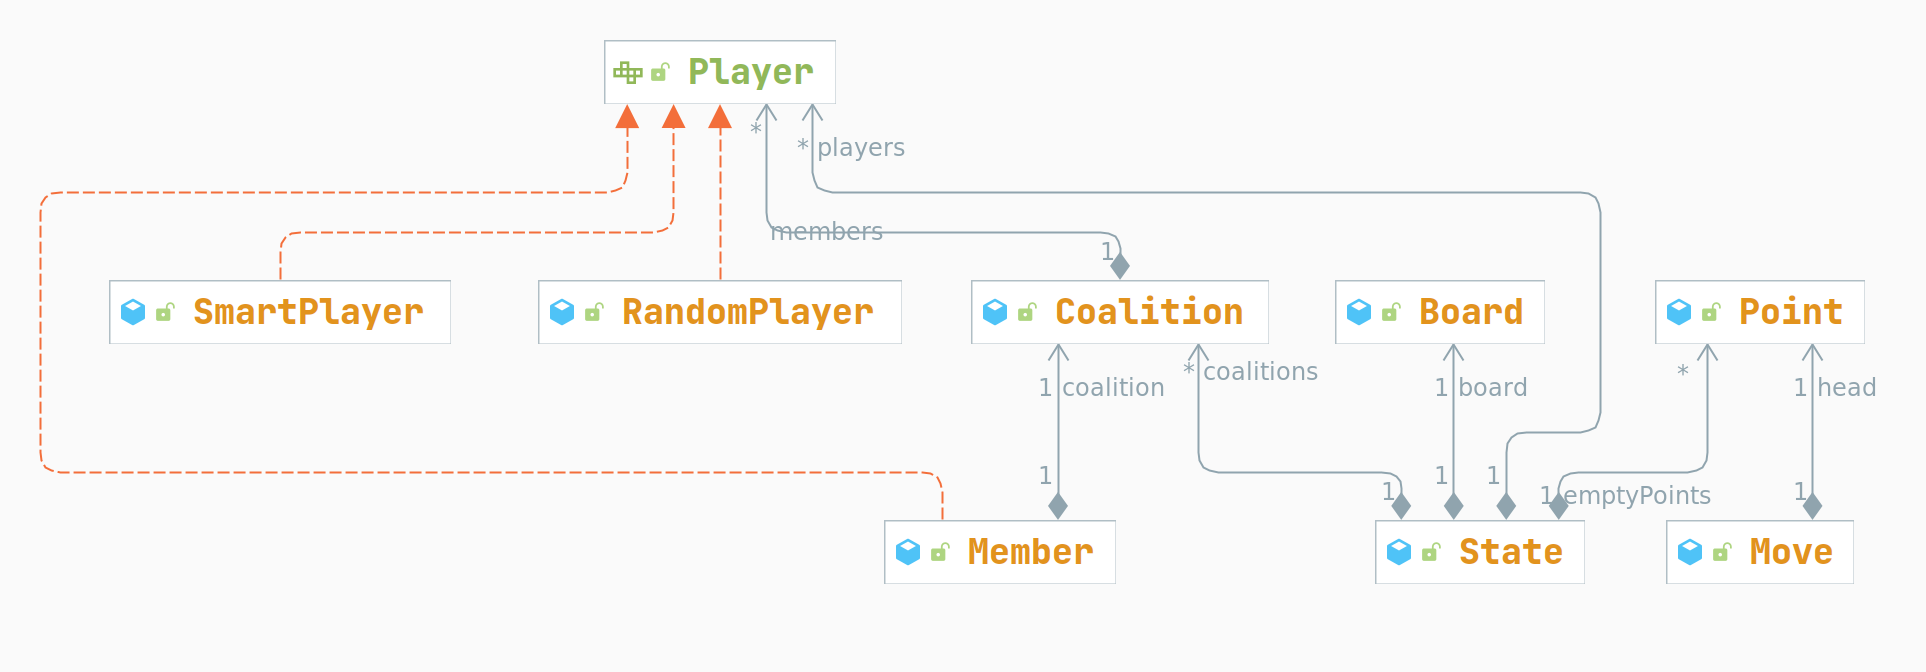
\includegraphics[scale=0.25]{diagrames/model}
	\caption{Diagramme de classe du modèle}
	\label{fig:modele}
\end{figure}\\


\tocless\paragraph{Move}
La classe Move est une classe importante de notre modèle qui représente le mouvement effectué par un joueur. Elle contient les 
informations nécessaires pour décrire un mouvement, à savoir la position final du joueur(dans notre cas la tête du joueur), la direction du mouvement et la longueur du mouvement qui a été effectué dans la même direction.
\begin{figure}[ht!]
	\centering
	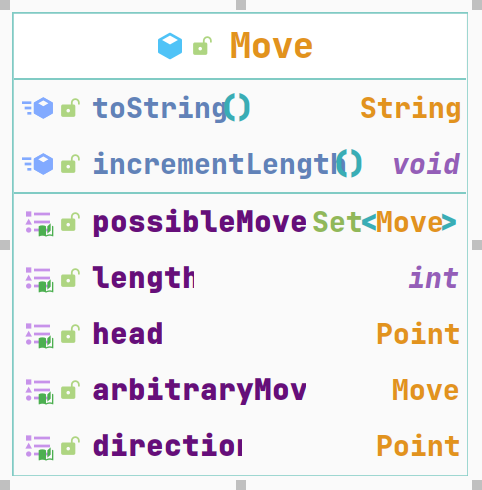
\includegraphics[scale=0.4]{diagrames/Move}
	\caption{Diagramme de classe de la classe Move}
	\label{fig:move}
\end{figure}
Grâce aux méthodes de la \classname{Move}(voir figure~\ref{fig:move}), on peut effectuer la validation d'un mouvement, obtenir la position final d'un mouvement, obtenir la direction d'un mouvement, obtenir la longueur d'un mouvement, etc.\\

Le choix de stocker la longueur d'un mouvement dans la classe \classname{Move}  découle du besoin de stocker les mouvements des joueurs dans une liste. 
En effet en considérant les mouvements effectués par le joueur rouge dans la figure~\ref{fig:heuristique},  si on stockait 
chaque position à un temps donné, on aurait eu besoin de stocker 20 éléments pour reconstituer le chemin du joueur rouge. Cependant, en utilisant notre implémentation, nous n'avons 
besoin de stocker que 9 mouvements, ce qui permet d'optimiser l'utilisation de la mémoire de notre application.\\

\tocless\paragraph{State}
La classe \classname{State} représente l'état du jeu à un instant donné. Elle contient les informations nécessaires pour décrire l'état du jeu(voir figure~\ref{fig:state}).
\begin{figure}[ht!]
	\centering
	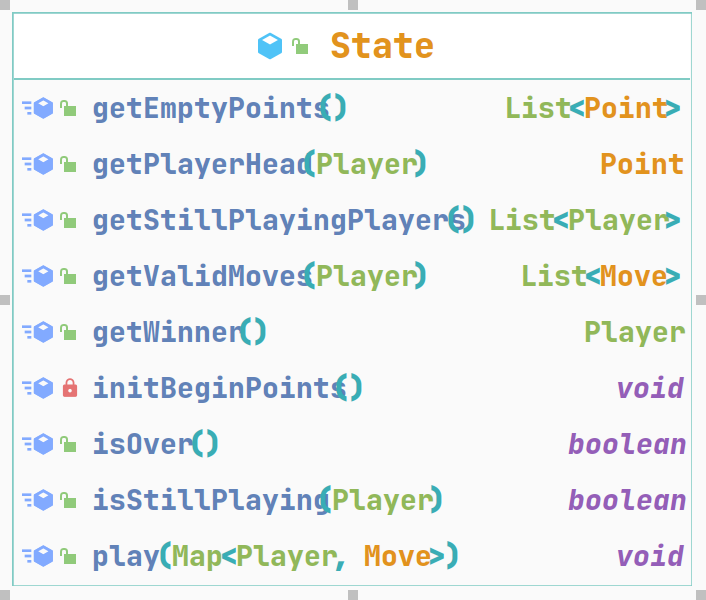
\includegraphics[scale=0.4]{diagrames/State}
	\caption{Diagramme de classe de la classe State}
	\label{fig:state}
\end{figure}\\

À travers cette classe, nous fournissons un objet permettant non seulement de pouvoir l'utiliser dans les algorithmes de recherche adversarial, mais aussi de pouvoir l'utiliser dans l'interface graphique pour afficher l'état du jeu.\\

L'une des principales méthodes de cette classe est la méthode \methodname{initBeginPoints} qui permet d'initialiser les positions initiales des joueurs.
Cette méthode est appelée dans le constructeur de la classe \classname{State} et permet de définir les positions initiales des joueurs. Pour un souci d'équitabilité, 
nous avons décidé de placer les joueurs de manière equidisante de centre du plateau de jeu. C'est à dire:
\begin{multline}
	\forall i ~\in ~$[0, nbJoueurs[$\\
	pos_x(i) = \frac{width}{2} + \frac{width}{2} \times \frac{2\pi i}{nbJoueurs}\\
	pos_y(i) = \frac{height}{2} + \frac{height}{2} \times \frac{2\pi i}{nbJoueurs}\\
\end{multline}
où $width$ et $height$ sont les dimensions du plateau de jeu et $nbJoueurs$ est le nombre de joueurs.\\

\subsubsection{Vue}
vue de l'application comporte des classes spécialement conçues pour faciliter l'interaction avec l'interface graphique 
utilisateur et pour offrir une représentation visuelle détaillée du déroulement des algorithmes et des parties. Elle permet à l'utilisateur de 
suivre les différentes étapes de l'exécution des algorithmes, de visualiser les mouvements des joueurs et d'observer le plateau de jeu de manière plus détaillée. 
En conséquence, la vue améliore significativement la compréhension et l'expérience de l'utilisateur lors de l'utilisation de l'application.

\tocless\paragraph{Les popups}
Les popups sont des éléments de l'interface graphique utilisateur qui sont utilisés pour fournir des informations supplémentaires à l'utilisateur ou 
pour les inviter à effectuer une action. Dans notre application, nous les avons utilisés pour afficher les informations relatives à la partie en cours tel que 
la fin de la partie, le gagnant, le nombre de coups joués(voir figure~\ref{fig:popupendgame}), etc.\\

\begin{figure}[H]
	\centering
	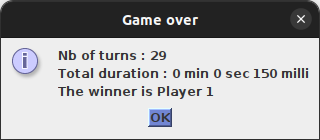
\includegraphics[scale=0.4]{Images/finjeu}
	\caption{Popup de fin de partie}
	\label{fig:popupendgame}
\end{figure}

En outre,  nous avons utilisé des fenêtres contextuelles pour permettre à l'utilisateur d'instancier les différentes IA qui s'affronteront sur le plateau et voir le récapitulatif global(voir figure~\ref{fig:fenetrecontextuelle}).
\begin{figure}[H]
	\centering
	\includegraphics[scale=0.4]{Images/récapitulatif}
	\caption{Fenêtre contextuelle}
	\label{fig:fenetrecontextuelle}
\end{figure}
Cette fonction est particulièrement utile car elle permet à l'utilisateur de sélectionner et de modifier les paramètres des différentes IA, tels que leur profondeur 
ou leur fonction heuristique. En fournissant ces fenêtres contextuelles, nous sommes en mesure d'améliorer l'expérience de l'utilisateur et de rendre l'application plus conviviale et intuitive.

\tocless\paragraph{La fenêtre de jeu}
La fenêtre principale du jeu sert d'interface principale pour afficher l'état actuel du jeu. Elle se compose de trois parties principales(voir figure~\ref{fig:fenetrejeu})

\begin{figure}[H]
	\centering
	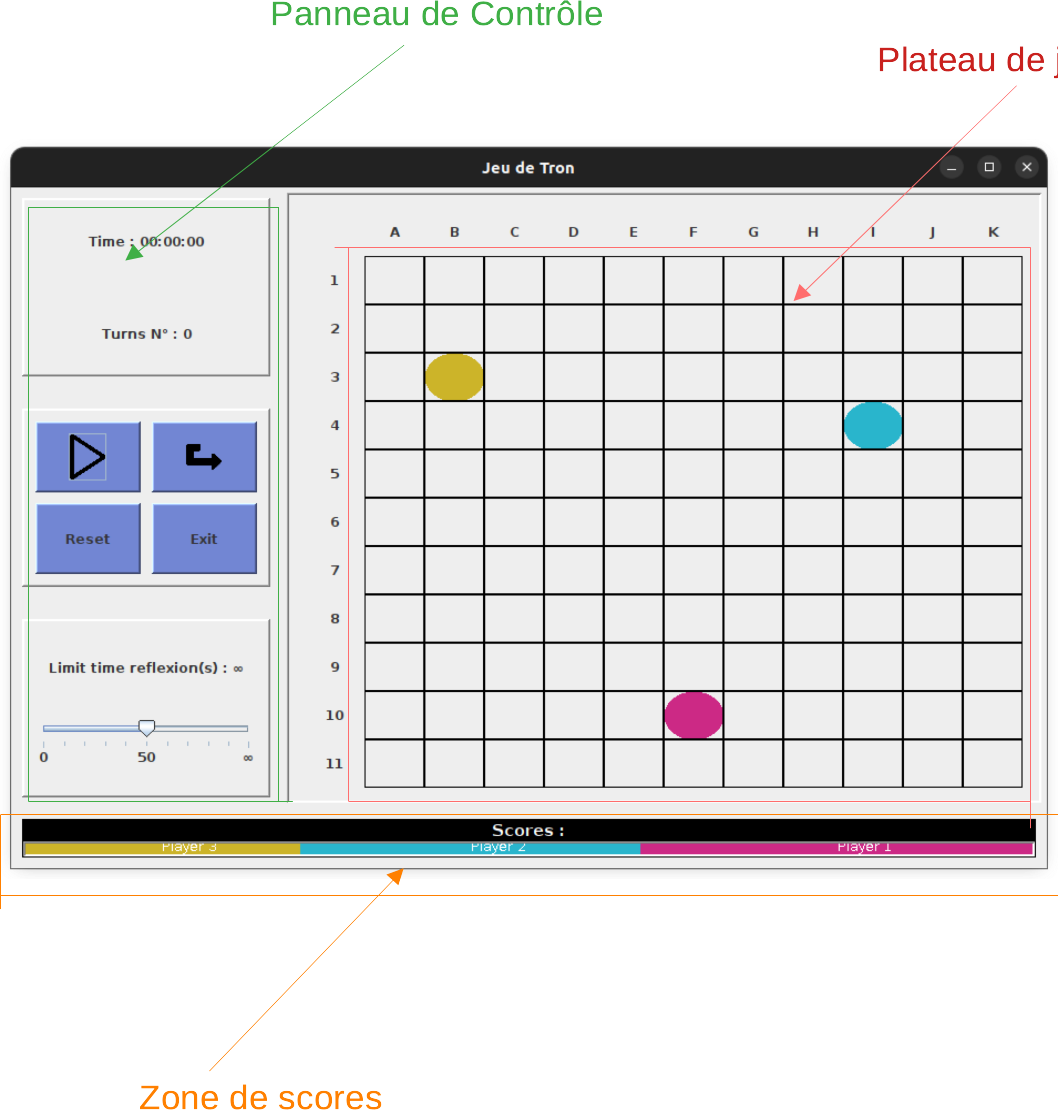
\includegraphics[scale=0.35]{Images/fenetrejeu}
	\caption{Fenêtre principale du jeu}
	\label{fig:fenetrejeu}
\end{figure}

Le plateau de jeu est une grille qui représente le terrain de jeu et affiche la position actuelle des joueurs. La zone de score fournit une représentation graphique de la zone 
occupée par chaque joueur sous la forme d'un graphique à barres. Le panneau de contrôle contient divers boutons et commandes, notamment les boutons de démarrage, de réinitialisation et 
d'étape suivante, ainsi que des informations sur le nombre de tours, la durée du jeu et un curseur permettant d'ajuster le temps de réflexion d'un algorithme.\\

\subsubsection{Algorithmes}
Le package \packagename{algorithms}  contient tous les algorithmes spécifiques que nous avons mis en œuvre pour le jeu(voir figure~\ref{fig:algorithms}).
\begin{figure}[H]
	\centering
	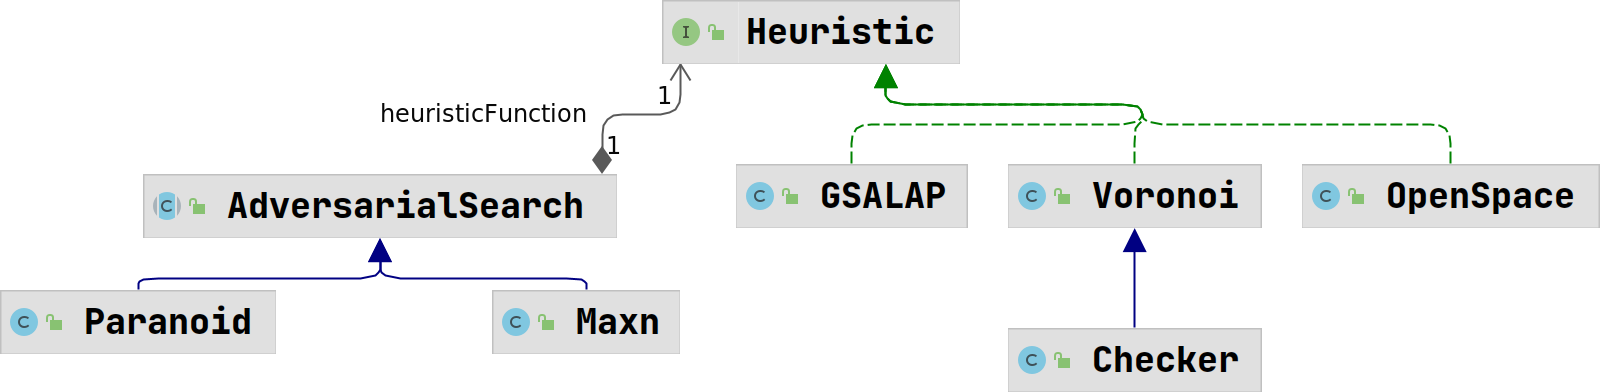
\includegraphics[scale=0.3]{diagrames/algorithms}
	\caption{Diagramme de classe du package algorithms}
	\label{fig:algorithms}
\end{figure}

Ces algorithmes sont classés en deux catégories :
\begin{itemize}
	\item les algorithmes de recherche adversarial
	\item les heuristiques(voir section~\ref{sec:analyse})\footnote{Les heuristiques sont utilisées pour évaluer les états du jeu et les comparer entre eux. Elles sont utilisées par les algorithmes de recherche adversarial pour
	déterminer le meilleur mouvement à effectuer.}
\end{itemize}

\subsection{Les fonctionnalités}
L'application offre diverses fonctionnalités qui permettent à l'utilisateur d'interagir avec le jeu, les algorithmes et l'interface. 
Les principales fonctionnalités sont les suivantes :
\begin{itemize}
	\item \textbf{Configuration de la partie} : : l'utilisateur peut configurer le jeu en définissant la taille du plateau, le nombre de joueurs et les algorithmes à utiliser.
	\item \textbf{Coloration d'un joueur} : Une couleur est attribuée à chaque joueur(couleur aléatoire variant d'une partie à l'autre) et est utilisée pour représenter le joueur sur le plateau de jeu.
	\item \textbf{Contrôle du jeu} : l'utilisateur peut démarrer, mettre en pause, reprendre et réinitialiser le jeu. L'utilisateur peut également avancer dans le jeu un coup à la fois.
	\item \textbf{Configuration des joueurs} : On peut configurer le temps de réflexion, la profondeur maximale de la recherche et les poids des heuristiques utilisées dans les algorithmes.
	\item \textbf{Sélection des algorithmes} : l'utilisateur peut choisir les algorithmes(recherche adversarial et heuristique) à utiliser pour chaque joueur.
	\item \textbf{Visualisation} : l'utilisateur peut visualiser les mouvements des joueurs et les étapes de l'exécution des algorithmes.
	\item \textbf{Statistiques du jeu} : l'application affiche diverses statistiques pendant et après le jeu, telles que le nombre de coups, la durée du jeu et les scores de chaque joueur.
	\item \textbf{Personnalisation de l'interface utilisateur} : l'utilisateur peut personnaliser l'interface utilisateur notamment en redimensionnant la fenêtre principale du jeu.
\end{itemize}







\section{Expérimentations et Évaluation}
\input{inputs/experimentations.tex}
\addcontentsline{toc}{section}{Conclusion et perspectives}
\section*{Conclusion et perspectives}
En conclusion, notre projet a exploré l'utilisation des algorithmes Maxn et paranoïaque dans le contexte d'un jeu multijoueur, et a montré que le choix de l'algorithme peut avoir un impact significatif sur la performance du joueur. Nos expériences ont démontré que l'algorithme paranoïaque est un concurrent de taille pour les jeux multijoueurs, surpassant l'algorithme Maxn dans certains cas.

Pour ce qui est de l'avenir, il existe plusieurs directions intéressantes dans lesquelles ce projet pourrait être étendu. L'une d'entre elles consisterait à étudier les performances des algorithmes Maxn et paranoïaque dans d'autres jeux multijoueurs que ceux que nous avons testés, tels que Tron. En particulier, le jeu Tron est un bon candidat pour une exploration plus approfondie car il présente un type de défi différent en ce qui concerne la stratégie et le mouvement, et nécessite donc des approches différentes de la conception et de l'optimisation des algorithmes.

Dans l'ensemble, notre projet a contribué à une meilleure compréhension des défis et des opportunités présentés par les jeux multijoueurs, et a démontré le potentiel des techniques algorithmiques avancées pour améliorer les performances des joueurs. Nous pensons que ce travail intéressera aussi bien les chercheurs que les développeurs de jeux, et nous sommes impatients de voir l'impact qu'il aura sur le domaine dans les années à venir.

\newpage
\addcontentsline{toc}{section}{Annexes}
\section*{Annexes}
\renewcommand{\thesection}{\Alph{section}}
\setcounter{section}{0}

% Analyse des heuristiques




\thispagestyle{empty}
%page des figures
\listoffigures

%page des tableaux
\listoftables

%page des algorithmes
\listofalgorithms

\addcontentsline{toc}{section}{Bibliographie}
\section*{Bibliographie}
\nocite{*}
\bibliographystyle{plain}
\bibliography{bibliography.bib}
\end{document}